\documentclass[10pt]{article}
\usepackage{tmlr}
% Camera-ready: \usepackage[accepted]{tmlr}   Preprint/arXiv: \usepackage[preprint]{tmlr}

\usepackage{hyperref}
\hypersetup{colorlinks=true, citecolor=blue!60!black, linkcolor=blue!60!black, urlcolor=blue!60!black}
\usepackage{float}
\usepackage{url}
\usepackage{amsmath,amssymb}
\usepackage{graphicx}
\usepackage{booktabs}
\usepackage{multirow}
\usepackage{array}
\usepackage{xcolor}
\usepackage{tikz}
\usetikzlibrary{positioning,arrows.meta,calc}

\newcommand{\AcapB}{A{\cap}B}
\newcommand{\AcapC}{A{\cap}C}
\newcommand{\BcapC}{B{\cap}C}
% Visible notes for the author. Remove every \authornote before submitting.
\newcommand{\authornote}[1]{\textcolor{red}{\textbf{[Author: #1]}}}

\title{Do Small Vision-Language Models Route Language the Same Way in Pixels and in Tokens? A Mechanistic Investigation with Code-Switched Text}

\author{\name Akshata \email akshatavidisha@gmail.com}

\def\month{MM}
\def\year{YYYY}
\def\openreview{\url{https://openreview.net/forum?id=XXXX}}

\begin{document}

\maketitle

% ============================================================
\begin{abstract}
Vision-language models (VLMs) increasingly read text as pixels, including code-switched text such as a screenshot of a Hinglish tweet, yet it is unknown whether the attention heads that matter for a language when it arrives as text tokens are the same ones that matter when it arrives as a rendered image. We investigate this in four open VLMs under 3B parameters. We score attention heads with gradient-based head importance (LAHIS) on monolingual English, Spanish, and Hindi sentences presented in three conditions (as text, as a rendered image with a query, and as a rendered image alone), probe the vision encoders for script identity on rendered Hindi-English code-switched sentences, and ablate the top-scoring heads while the models read code-switched images. The answer depends on the model. In Qwen2-VL-2B and SmolVLM, text and image inputs recruit largely different heads (text-image Jaccard overlap 0.05--0.21, against 0.43--0.91 between the two image conditions). In InternVL3-2B they nearly coincide, but only for Hindi (0.667). For PaliGemma-3B the overlap measure cannot distinguish either pattern from chance. All four vision encoders separate Latin from Devanagari script from their first layer, with peak balanced accuracy from 0.63 to 0.99. Zero-ablating the top Hindi heads changes the script of the output far more often than ablating random heads in Qwen2-VL-2B (70\% vs.\ 7\% of outputs) and PaliGemma-3B (97\% vs.\ 7\%). In SmolVLM, ablation breaks generation rather than redirecting it, and in InternVL3-2B, the model whose heads overlap most across modalities, the effect is not distinguishable from the control. We report these results as a per-model map rather than a general law, and release the pipeline, the corpus, and the per-head scores.
\end{abstract}

% ============================================================
\section{Introduction}
\label{sec:intro}

A phone screenshot of a Hinglish tweet, a photographed handwritten note, and a chat screenshot pasted into a vision-language assistant all put the same problem to a VLM. It has to identify and route two languages within a single image, without the token-level segmentation a text-only language model gets for free.

A VLM has two main parts. A vision encoder turns an image into a sequence of tokens, much as a tokenizer turns text into a sequence of tokens. A language decoder then reads whichever tokens it is given, whether they came from text or from the vision encoder, and generates output text. The same decoder can therefore meet the same sentence along two different paths. Whether its attention heads handle the sentence the same way on both paths is not known.

Prior mechanistic work on multilingual routing has focused almost exclusively on the text-only case. \citet{liu2026lahis} introduce Language Attention Head Importance Scores (LAHIS) and show that a small set of attention heads in multilingual LLMs matters far more than the rest for language identification, discoverable via a single forward-backward pass with a differentiable head mask. \citet{nie2025confusion} trace language-confusion failures in English-centric LLMs to specific ``confusion point'' positions and final-layer transitions. \citet{wendler2024llamas} show that intermediate Llama-2 representations are closer to an English pivot than to the input or output language. On the vision-language side, \citet{ye2025claim} identify cross-lingual attention misalignment in VLMs and intervene on it to reduce multilingual object hallucination, and \citet{baek2025ocr} characterize ``OCR heads'' responsible for reading text embedded in images, but restrict their study to English text on English-centric models.

The question matters for how far existing interpretability work already takes us. If a VLM routes a sentence through the same heads whether it arrives as text or as pixels, findings about language heads from text-only work should carry over to the visual case. If the two paths use different heads, the visual path needs to be studied on its own. Motivated by this gap, we investigate two research questions and one exploratory question:

\begin{itemize}
    \item \textbf{RQ1: Do text and image inputs share language-routing heads?} When the same sentence reaches a VLM as text tokens and as a rendered image, are the most important attention heads the same?
    \item \textbf{RQ2: Are the identified heads causally involved?} When a VLM reads code-switched text from an image, does ablating the heads that gradient attribution ranks highest change the language of its output, beyond what ablating random heads does?
    \item \textbf{Exploratory: Does the base decoder shape which heads matter?} Across models, do the important head positions track the decoder family, the vision encoder, or language competence?
\end{itemize}

Before answering these, we check a precondition: whether script identity (Latin vs.\ Devanagari) is even available in the vision encoder's representations. If it were not, a divergence between the text and image paths would be unsurprising.

\paragraph{Where code-switching enters.}
Following \citet{liu2026lahis}, we identify important heads on monolingual sentences, one language at a time, so the head sets for RQ1 come from monolingual English, Spanish, and Hindi text. Code-switched text enters in two places: the script probes, which read mixed-script images, and the causal test in RQ2, which asks whether heads identified on monolingual text change what a model produces when it reads a code-switched image. Identifying heads directly on code-switched sentences is left to future work (Section~\ref{sec:limitations}).

\paragraph{What we find.}
Script identity is linearly decodable from the first layer of all four vision encoders, with peak balanced accuracy from 0.63 to 0.99 (Section~\ref{sec:probes}). The answer to RQ1 differs by model: two models use largely separate heads for text and image input, one nearly shares them for Hindi only, and for one the measure is inconclusive (Section~\ref{sec:overlap}). For RQ2, ablating the top heads changes the output script far more than ablating random heads in two models. In a third, ablation breaks generation, so the flip metric is uninformative, and in the model whose text and image heads overlap most the effect is not distinguishable from the control (Section~\ref{sec:ablation}). For the exploratory question, the two models with a shared decoder family share 18 of their top 20 head positions, but most of that match is expected from both models placing their top heads in the same two layers (Section~\ref{sec:lineage}).

\paragraph{Scope.}
This is an investigative study of four small VLMs, two language pairs, and one attribution method. We report what happens in each model and state how strong the evidence is for each observation (Section~\ref{sec:conclusions_table}). We do not claim that the patterns generalize to other VLMs.

% ============================================================
\section{Related Work}
\label{sec:related}

\paragraph{Language-specific heads and neurons in text LLMs.}
Beyond LAHIS, \citet{tang2024neurons} identify language-specific neurons via parallel-corpus activation contrasts and show that deactivating them degrades only the corresponding language. \citet{wendler2024llamas} probe intermediate representations directly for an English-pivot signature. This line of work establishes that language routing in LLMs is sparse, identifiable, and at least partially causal. It is, however, entirely text-only. None of it asks what happens when the same content is presented as an image instead of a token sequence.

\paragraph{Code-switching circuits.}
\citet{nie2025confusion} is the closest prior work to a mechanistic study of multilingual routing failure, localizing language-confusion errors to specific token positions and late-layer transitions in text-only models. We are not aware of any prior mechanistic study of code-switching specifically (as opposed to single-language confusion), and none that touches the visual modality.

\paragraph{Language heads in VLMs.}
\citet{ye2025claim} (CLAIM) is the closest prior work to ours. It identifies cross-lingual attention misalignment in VLMs and intervenes on it. The critical differences are that CLAIM studies monolingual queries in different languages rather than code-switched content, and it does not isolate the text path from the vision path, so it cannot ask whether a VLM's \emph{text} decoder and its \emph{image-reading} decoder agree on which heads matter. \citet{baek2025ocr} characterize OCR heads in VLMs but restrict their study to English text, leaving open whether script-mixed or language-mixed visual text is routed any differently.

\paragraph{Reading text from pixels.}
Several models process text directly as rendered images, including pixel-based language models \citep{rust2023pixel}, a single encoder for images and rendered text \citep{tschannen2023clippo}, and OCR-free document and screenshot understanding \citep{kim2022donut, lee2023pix2struct}. On the vision-encoder side, work on CLIP shows that image encoders represent written words separately from the scenes they appear in \citep{materzynska2022disentangling}, and that individual attention heads in CLIP's image encoder specialize in specific, interpretable image properties \citep{gandelsman2024interpreting}. Our script probes (Section~\ref{sec:probes}) ask a narrower version of this question for the encoders inside VLMs.

\paragraph{Where visual information enters the decoder.}
Mechanistic work on VLMs has begun to trace how image information reaches and moves through the language model, using causal tracing \citep{palit2023towards, basu2024understanding} and by following how visual tokens are processed across layers \citep{neo2025towards}. These studies localize visual information flow, but none asks whether the heads that matter for a language when it is read from an image are the same heads that matter when it is read as text.

\paragraph{Gap.}
To our knowledge, no prior work compares which attention heads a VLM relies on for the same sentence as text and as a rendered image, at head-level granularity and with the effect of the text query separated from the effect of modality, or tests those heads on code-switched images.

% ============================================================
\section{Data}
\label{sec:data}

All code-switched text is real and human-produced, with gold token-level language labels. We avoid synthetic code-switching, such as naive word substitution, since it risks sentences no bilingual speaker would actually write.

Hindi-English data comes from the Devanagari-script Twitter portion of the GLUECoS part-of-speech corpus \citep{khanuja2020gluecos}, and Spanish-English data comes from the Bangor Miami corpus of transcribed bilingual speech \citep{deuchar2013bangor}. Monolingual baselines in English, Spanish, and Hindi come from FLORES-200 parallel triples.

\paragraph{Cleaning and final counts.}
We clean the raw social-media and transcribed-speech text with Penn Treebank detokenization, script- and noise-consistency filters, a two-stage fluency filter (heuristic checks, then Qwen2.5-0.5B perplexity, dropping the worst quartile per language pair), and a content filter for profanity and political material judged by Claude against a fixed rubric, keeping every dropped record's drop reason for auditability.

After filtering, the corpus contains 933 code-switched sentences (806 Hindi-English, 127 Spanish-English), 118 natural Hindi-English sentences from a separate test split, disjoint from that set, 750 monolingual sentences (250 per language), and 100 Hindi-in-Latin-script transliteration controls, which separate script identity from language identity since this content is Hindi written in the Latin alphabet.

\paragraph{Which data each analysis uses.}
\begin{itemize}
    \item \textbf{Head importance (RQ1).} For each language, 100 of the 250 monolingual FLORES sentences. Each sentence is entirely in one language, and the loss covers all of its tokens. Conditions B and C use rendered images of the same sentences. No code-switched text is used to identify heads.
    \item \textbf{Script probes.} Rendered Hindi-English code-switched sentences, whose per-token bounding boxes give each image patch a script label.
    \item \textbf{Hindi-English ablation (RQ2).} 100 sentences sampled from the 806 Hindi-English code-switched sentences. Because heads are identified on FLORES, these images are disjoint from the data used to select heads.
    \item \textbf{Spanish-English ablation.} The first 100 of the 127 Spanish-English code-switched sentences, likewise disjoint from the FLORES head-scoring sentences.
\end{itemize}

\paragraph{Rendering.}
Every sentence exists as both raw text and a rendered image, black text on a white canvas, with per-token bounding boxes so patch-level attention can later be mapped back to source-language spans. Code-switched sentences render each token in a script-appropriate font, Noto Sans for Latin and Noto Sans Devanagari for Devanagari, so script boundaries are visually real rather than assumed. Figure~\ref{fig:stimuli} shows sample rendered stimuli. Hindi-English items mix Devanagari and Latin script within a sentence; Spanish-English items stay in Latin script throughout, which is why the script-flip metric (Section~\ref{sec:ablation_method}) applies only to the Hindi-English pair.

\begin{figure}[t]
\centering
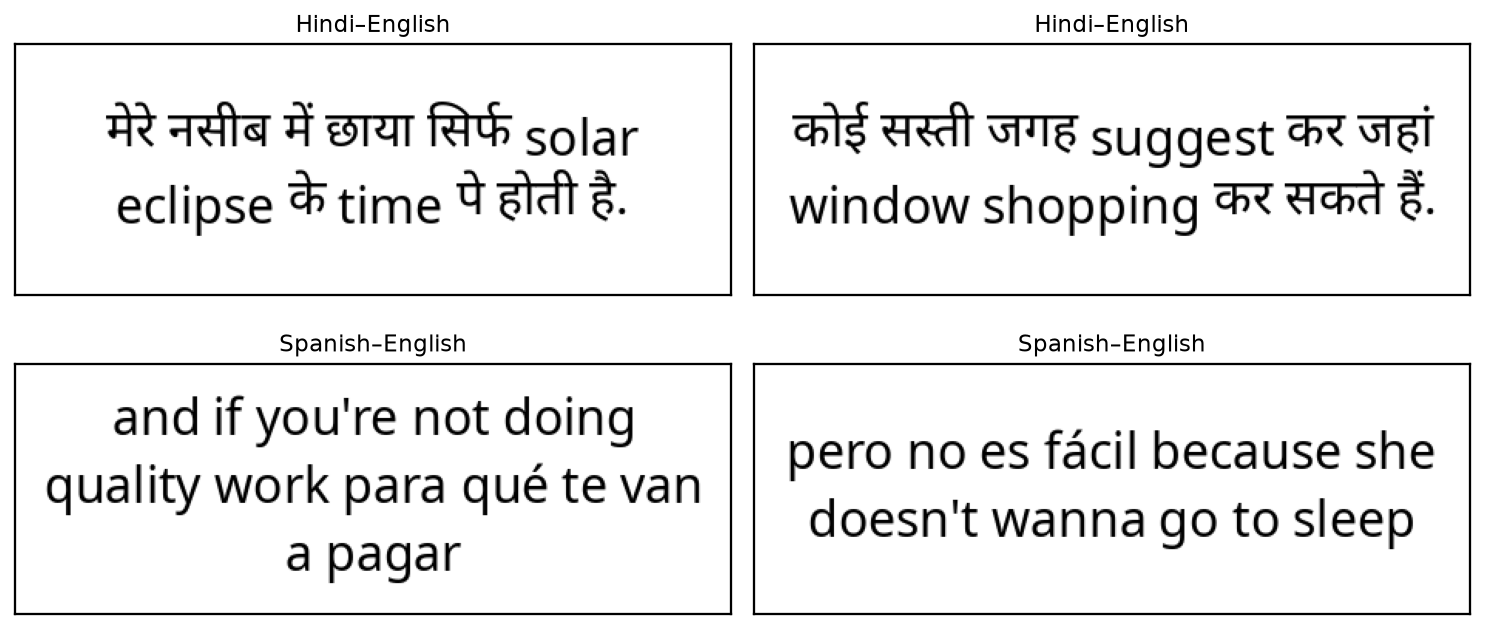
\includegraphics[width=0.85\linewidth]{figures/sample_stimuli.png}
\caption{Four rendered code-switched sentences from the evaluation set (two Hindi--English, two Spanish--English), shown as the models see them, rendered to an image with no accompanying prompt tokens.}
\label{fig:stimuli}
\end{figure}


% ============================================================
\section{Models}
\label{sec:models}

We evaluate four open VLMs, chosen to differ in vision encoder, decoder family, and image-token compression scheme while remaining small enough (1.7--3B total or decoder parameters) to run full LAHIS gradient attribution (forward and backward passes with a per-head soft mask) on the hardware available to us, a single NVIDIA T4 GPU with 16GB of VRAM. Model size was chosen to fit this budget, not for any property of the models themselves.

\begin{itemize}
    \item \textbf{Qwen2-VL-2B-Instruct} \citep{wang2024qwen2vl} pairs a custom 2D-RoPE vision transformer (0.67B) with a $2{\times}2$ patch-merger and a Qwen2-1.5B decoder (28 layers, 12 attention heads).
    \item \textbf{InternVL3-2B} \citep{chen2024internvl} pairs InternViT-300M (v2.5), with pixel-shuffle compression, and a Qwen2.5-1.5B decoder (28 layers, 12 attention heads).
    \item \textbf{SmolVLM-Instruct} \citep{marafioti2024smolvlm} pairs a SigLIP-SO400M \citep{zhai2023sigmoid} vision encoder and a fixed-scale-factor pixel-shuffle connector with a SmolLM2-1.7B decoder (24 layers, 32 attention heads).
    \item \textbf{PaliGemma-3B (mix-448)} \citep{beyer2024paligemma} pairs a SigLIP-SO400M vision encoder at 448px and a linear projector that keeps all 1024 image tokens (no merging or pooling) with a Gemma-2B decoder (18 layers, 8 attention heads, multi-query attention). It is a \emph{prefix-LM}, so image and prompt tokens receive bidirectional attention and only the suffix is trained causally. We therefore score its decoder in that native suffix regime, taking the loss on the text tokens of \texttt{[BOS]\,\textbackslash n\,text}, for both the competence gate and the LAHIS A condition.
\end{itemize}

Qwen2-VL-2B and InternVL3-2B share a decoder family (Qwen2 and Qwen2.5). To our knowledge, Qwen2.5 is a separate pretraining run in that family rather than a continuation of Qwen2's weights \citep{qwen2024qwen25}, so the two decoders share architecture and training recipe but not weights. SmolVLM's SmolLM2 decoder is Llama-architecture and PaliGemma's is Gemma, each from an unrelated pretraining lineage. The exploratory analysis in Section~\ref{sec:lineage} uses this structure.

\paragraph{Language competence gate.}
Before running any language-routing analysis, we verify that each extracted decoder is competent in each language, so that head-importance scores do not measure noise. We compute decoder perplexity on monolingual FLORES text (Table~\ref{tab:competence}), using a per-token threshold of 100. All four models pass, though PaliGemma-3B's per-token Spanish (114.7) slightly exceeds it.

Per-token perplexity must not be compared across languages, because tokenizer fertility differs by 3.4 to 3.6 times between English (about 0.23 tokens per character) and Devanagari Hindi (about 0.78). This mechanically deflates Hindi's per-token perplexity regardless of competence. We therefore normalize by characters, using $\mathrm{ppl}_c = \exp(\mathrm{NLL}/n_{\mathrm{chars}})$. On this scale Hindi is the hardest language for every model, and all cross-language competence statements in this paper use the character-normalized values.

\begin{table}[t]
\centering
\caption{Decoder language competence on monolingual FLORES text. Per-token perplexity is deflated for Hindi by tokenizer fertility and is not comparable across languages. The character-normalized values are comparable and show Hindi is hardest for every model, with all models in range. PaliGemma-3B is scored in its native prefix-LM regime.}
\label{tab:competence}
\begin{tabular}{l ccc c ccc}
\toprule
& \multicolumn{3}{c}{Per-token ppl.} && \multicolumn{3}{c}{Char.-normalized ppl.} \\
\cmidrule(lr){2-4} \cmidrule(lr){6-8}
Model & en & es & hi && en & es & hi \\
\midrule
Qwen2-VL-2B  & 40.9 & 26.2  & 5.9  && 2.06 & 2.23 & 4.46 \\
InternVL3-2B & 38.4 & 28.0  & 6.7  && 2.04 & 2.28 & 4.87 \\
SmolVLM      & 83.8 & 49.5  & 7.4  && 2.23 & 2.98 & 7.64 \\
PaliGemma-3B & 91.3 & 114.7 & 69.4 && 2.48 & 2.75 & 4.48 \\
\bottomrule
\end{tabular}
\end{table}

% ============================================================
\section{Method}
\label{sec:method}

Figure~\ref{fig:pipeline} gives an overview of this pipeline before we describe each part in detail.

\begin{figure}[t]
\centering
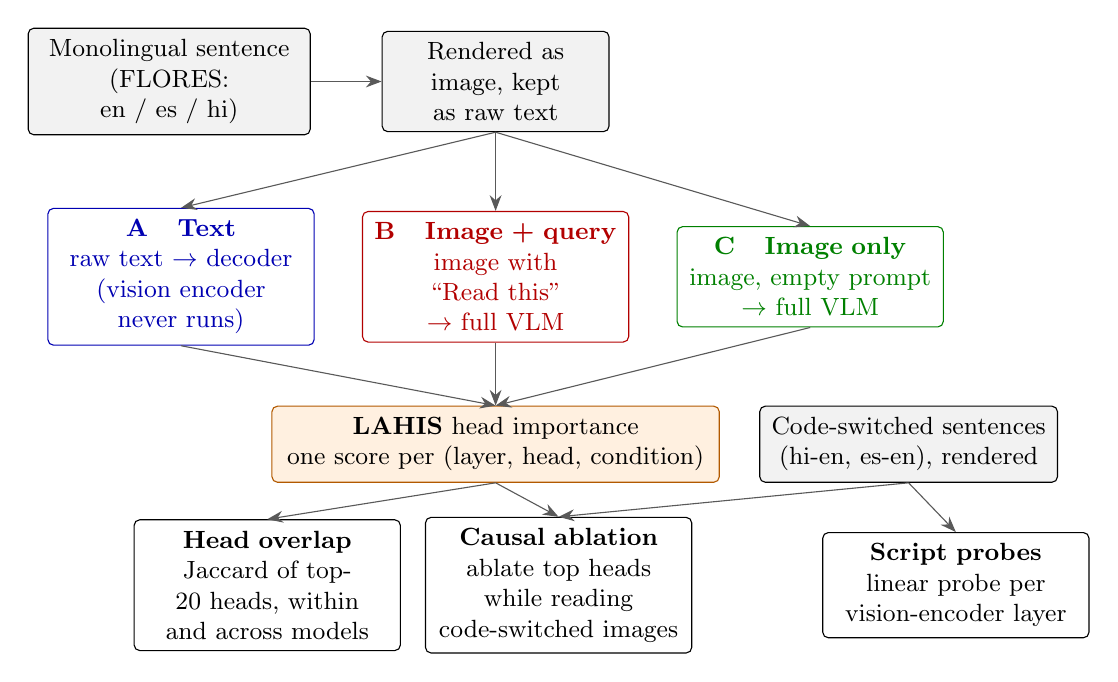
\begin{tikzpicture}[
    font=\small,
    box/.style={draw, rounded corners=2pt, align=center, inner sep=4pt, minimum height=2.4em},
    arr/.style={-{Stealth[length=2mm]}, gray!70!black},
]
\node[box, fill=gray!10, text width=2.6cm] (rend) {Rendered as image, kept as raw text};
\node[box, fill=gray!10, text width=3.3cm, left=0.9cm of rend] (src) {Monolingual sentence\\(FLORES: en / es / hi)};

\node[box, draw=red!70!black, text=red!70!black, text width=3.1cm, below=1.0cm of rend] (B) {\textbf{B\quad Image + query}\\image with ``Read this''\\$\rightarrow$ full VLM};
\node[box, draw=blue!70!black, text=blue!70!black, text width=3.1cm, left=0.6cm of B] (A) {\textbf{A\quad Text}\\raw text $\rightarrow$ decoder\\(vision encoder never runs)};
\node[box, draw=green!50!black, text=green!50!black, text width=3.1cm, right=0.6cm of B] (C) {\textbf{C\quad Image only}\\image, empty prompt\\$\rightarrow$ full VLM};

\node[box, fill=orange!12, draw=orange!70!black, text width=5.4cm, below=0.8cm of B] (lahis) {\textbf{LAHIS} head importance\\one score per (layer, head, condition)};
\node[box, fill=gray!10, text width=3.5cm, right=0.5cm of lahis] (cs) {Code-switched sentences\\(hi-en, es-en), rendered};

\node[box, text width=3.1cm] (overlap) at ($(lahis.south)+(-2.9,-1.3)$) {\textbf{Head overlap}\\Jaccard of top-20 heads, within and across models};
\node[box, text width=3.1cm] (abl) at ($(lahis.south)+(0.8,-1.3)$) {\textbf{Causal ablation}\\ablate top heads while reading code-switched images};
\node[box, text width=3.1cm] (probe) at ($(cs.south)+(0.6,-1.3)$) {\textbf{Script probes}\\linear probe per\\vision-encoder layer};

\draw[arr] (src) -- (rend);
\draw[arr] (rend.south) -- (A.north);
\draw[arr] (rend.south) -- (B.north);
\draw[arr] (rend.south) -- (C.north);
\draw[arr] (A.south) -- (lahis.north);
\draw[arr] (B.south) -- (lahis.north);
\draw[arr] (C.south) -- (lahis.north);
\draw[arr] (lahis.south) -- (overlap.north);
\draw[arr] (lahis.south) -- (abl.north);
\draw[arr] (cs.south) -- (abl.north);
\draw[arr] (cs.south) -- (probe.north);
\end{tikzpicture}
\caption{Overview of the pipeline. Head importance is scored with LAHIS on monolingual sentences in three conditions (A, B, C), and the top heads are compared across conditions and models. Code-switched sentences, rendered as images, are used for the script probes and for the causal ablation, which removes the top heads while the model reads them.}
\label{fig:pipeline}
\end{figure}

\subsection{Three conditions}
\label{sec:conditions}

For each language and each sentence, we evaluate three conditions:

\begin{description}
    \item[A (text)] The extracted decoder processes the raw sentence text. This decoder is the language model submodule taken \emph{from inside} the VLM after its own vision-language instruction tuning, not a separately loaded checkpoint. The vision encoder never runs.
    \item[B (image+query)] The full VLM processes the rendered image plus a fixed textual instruction (``Read this:''), with the loss computed on the appended target sentence.
    \item[C (image-only)] Identical to B but with an empty instruction. It uses the same processor chat template as B (image block, user and assistant role tokens), with the user's text field left empty, so it adds no instruction-language tokens beyond the role tokens that B and C already share.
\end{description}

Comparing B with C isolates the effect of the text query, and comparing A with C isolates the effect of modality. Using the decoder \emph{extracted from} the VLM for condition A, rather than the original pre-finetuning checkpoint, is essential. It ensures that A vs.\ C isolates modality alone, without confounding modality with whether the weights have seen vision-instruction tuning at all.

\subsection{Head importance (LAHIS)}
\label{sec:lahis}

Following \citet{liu2026lahis}, we install a differentiable soft mask $M \in \mathbb{R}^{L \times H}$ (initialized to all ones) that multiplies each attention layer's per-head output via a forward pre-hook on the output projection. This works because the projection's \emph{input} is the concatenation of per-head outputs and can therefore be sliced exactly per head (unlike hooking the post-projection output, which mixes heads). We compute the language-modeling loss and take $|\partial \mathrm{loss}/\partial M|$ as the importance score for each head, averaged over 100 monolingual FLORES sentences per condition per language, with the loss taken over all tokens of each sentence (Section~\ref{sec:data}). This requires only one forward and one backward pass per sentence. We visualize these scores as layer$\times$head maps in Appendix~\ref{app:lahis}, for Hindi (Figure~\ref{fig:lahis_hi}) and Spanish (Figure~\ref{fig:lahis_es}).

\paragraph{What this score measures.}
The loss behind LAHIS is the ordinary next-token loss, not a loss tied to language identity. A head scores highly if removing it hurts prediction of text in the given language, which includes heads that do general work such as tracking position or copying earlier tokens. We therefore read a high score as ``important for processing this language'', not ``specific to this language''. Section~\ref{sec:lineage} shows that most top-scoring heads are indeed shared across all three languages within each model.

\subsection{Head overlap}
\label{sec:overlap_method}

For each model and language, we compute the top-20 heads by importance under each condition and report pairwise Jaccard overlap ($|A \cap B|/|A \cup B|$) between conditions. We additionally compute a 10{,}000-sample permutation baseline (randomly-drawn 20-head sets from the same layer$\times$head grid, computed separately per model since the grids differ in size) to establish chance-level overlap, and sweep $K \in \{5, 10, 20, 40, 80\}$ to check that our results are not an artifact of the specific top-20 cutoff.

For the exploratory cross-model analysis, we additionally record the raw (layer, head) coordinates in each model's top-20 text-condition set and compute pairwise coordinate overlap between every pair of models.

\subsection{Script probes}
\label{sec:probe_method}

To ask whether script identity is already linearly decodable inside the vision encoder, before any information reaches the decoder, we train balanced-accuracy logistic-regression probes (5-fold cross-validated) at every vision-encoder layer, predicting each patch's script (Latin, Devanagari, or background) from its frozen hidden state. Patch-to-script labels come from the token bounding boxes recorded at render time, mapped onto the actual grid of image tokens the decoder sees.

This grid differs from the raw patch grid whenever a compression module, such as a patch merger or pixel-shuffle layer, runs between encoder and decoder. Background patches are labeled only to be excluded. Every patch we actually fit or score the probe on is Latin or Devanagari, so the reported classifier is binary and chance is 0.5, not 1/3.

\subsection{Causal ablation}
\label{sec:ablation_method}

Head importance from gradient attribution is correlational. A head can receive a large gradient without being causally responsible for the model's output. We test causality directly by zero-ablating the top-20 heads found under condition A for English and for Hindi separately, via the same per-head output-projection hook, now clamping the targeted heads' output to zero, and generating text from each of 100 Hindi-English code-switched images (Section~\ref{sec:data}). Generation is greedy and deterministic (no sampling, 64-token budget), so ablation variants differ only in which heads are masked, not in decoding randomness.

We record whether the output script changes from the un-ablated baseline. We restrict this test to Hindi-English images because the outcome measure is a script change, and script is only informative when the two code-switched languages do not share one. Spanish-English is handled separately with a language-identification metric (Table~\ref{tab:es_ablation}).

The ablated sets are simply the 20 highest-scoring heads for each language, not heads that score higher for one language than the other. Because most top heads are shared across languages (Section~\ref{sec:lineage}), the English and Hindi sets overlap heavily, so ``Hindi heads'' and ``English heads'' name the language the heads were scored on rather than heads specific to that language.

We compare against two controls. The first is a random 20-head set, drawn from heads \emph{outside} the top-20 English and Hindi sets and redrawn for each seed, to test whether \emph{any} 20-head ablation changes output this much. The second is a mean-ablation variant, which replaces each head's output with its mean taken over token positions within that same image's baseline forward pass (per-sentence, per-head, not corpus-wide) rather than zero, to separate language-related suppression from generic degradation.

\paragraph{What this metric measures.}
A script flip records that the output \emph{switched} to the other script. Ablation can also damage the output without switching its script, for example by producing repeated or truncated text in the original script, and our metric does not register that. The flip rate is therefore a measure of how much ablation redirects the output language, not of how much it disrupts generation overall.

% ============================================================
\section{Results}
\label{sec:results}

\subsection{Precondition: script identity is decodable early in every vision encoder}
\label{sec:probes}

Script-probe balanced accuracy exceeds the 50\% chance level even at layer 0 for all four encoders, confirming script identity is present in the earliest patch embeddings before any contextualization across the image.

The four encoders differ substantially in how well. InternVL3-2B's InternViT reaches 0.990 balanced accuracy by layer 8 of 24 and stays above 0.98 through its final layer, near-perfect linear separability. PaliGemma-3B's SigLIP-SO400M encoder is nearly as strong, 0.982 at layer 12 of 27, climbing from an already-high 0.818 at layer 0. Qwen2-VL's custom encoder peaks lower, 0.811 at layer 12 of 32. SmolVLM's SigLIP-SO400M encoder is the weakest by a wide margin and, unlike the other three, never improves substantially with depth. It peaks at only 0.630 (layer 8 of 27) and \emph{declines} to 0.605 by its final layer.

PaliGemma-3B and SmolVLM share the same vision-encoder family (SigLIP-SO400M), yet sit at opposite extremes, 0.982 against 0.630. The two deploy it differently. PaliGemma runs SigLIP at 448px and keeps all 1024 patch tokens, whereas SmolVLM feeds it lower-resolution, pooled tokens. Within one encoder family, then, the script signal varies with resolution and token budget. All four models are given the same rendered images with the same fonts, so this spread comes from the encoders rather than the stimuli. Figure~\ref{fig:probes} shows the full per-layer trajectories.

\begin{figure}[t]
\centering
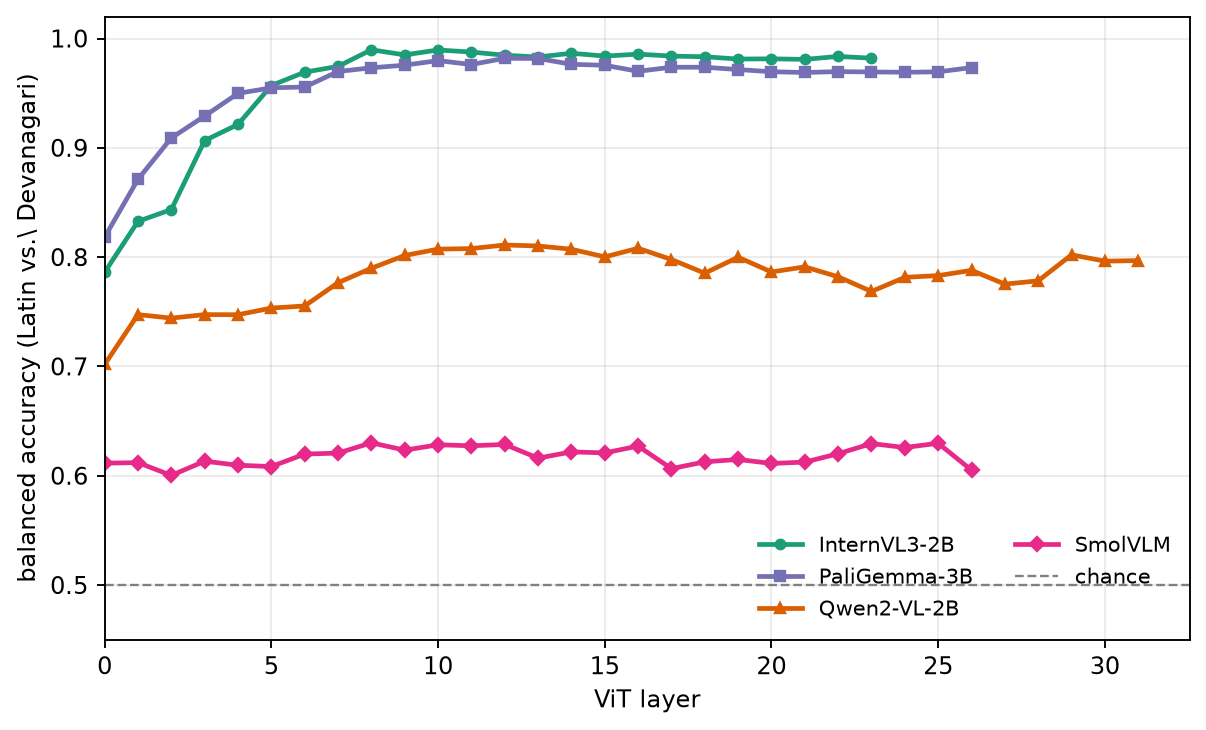
\includegraphics[width=0.62\linewidth]{figures/script_probes.png}
\caption{Script-probe balanced accuracy (Latin vs.\ Devanagari patches, 5-fold CV) at every vision-encoder layer, all four models (dashed line: chance, 0.5). InternVL3-2B and PaliGemma-3B both rise quickly and saturate near 1.0 (0.990 and 0.982 peak). Qwen2-VL-2B rises more slowly to a lower plateau (0.811). SmolVLM stays close to its layer-0 value throughout (0.630 peak), so its weak script separability is not a matter of needing more depth. PaliGemma and SmolVLM share the SigLIP-SO400M encoder family yet sit at opposite extremes (Section~\ref{sec:probes}).}
\label{fig:probes}
\end{figure}


These probes track rendered script rather than language content. We apply each model's already-trained, peak-layer Latin-versus-Devanagari probe to the 100 Hindi-in-Latin-script transliteration controls (Section~\ref{sec:data}), which are Hindi \emph{words} written in Latin \emph{glyphs}. The probe calls them Latin at a rate matching its own code-switched-data accuracy (InternVL3-2B 99.7\%, PaliGemma-3B 99.7\%, Qwen2-VL-2B 97.3\%, SmolVLM 84.0\%, against 98.8\%, 98.2\%, 80.2\%, and 62.4\% balanced accuracy on real script respectively). The probes read orthography, not the underlying language.

Script identity is therefore available to every decoder in the study. Where a model's text and image paths use different heads (Section~\ref{sec:overlap}), it is not because the encoder failed to separate the scripts.

\subsection{RQ1: whether text and image inputs share heads depends on the model}
\label{sec:overlap}

Figure~\ref{fig:overlap} plots, for each model and language, how much the top-20 heads for text overlap with those for the image alone ($\AcapC$), next to how much the two image conditions overlap with each other ($\BcapC$), against a permutation-derived chance level (95th percentile over 10{,}000 random 20-head draws). Table~\ref{tab:overlap} (Appendix~\ref{app:overlap}) gives all three pairwise overlaps. The four models show three different patterns.

\begin{figure}[t]
\centering
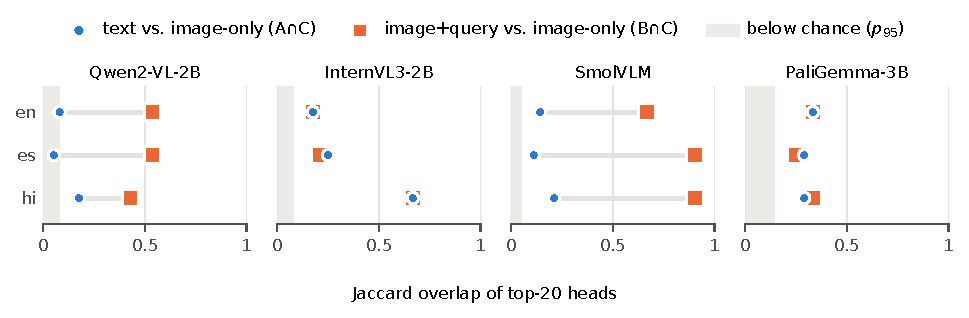
\includegraphics[width=\linewidth]{figures/overlap_dumbbell.pdf}
\caption{Do text and image inputs recruit the same heads? Each row compares text-vs-image overlap ($\AcapC$, circles) with image-vs-image overlap ($\BcapC$, squares) for one language. A long bar means the image conditions agree with each other but not with text. Where the markers coincide, text and image agree as much as the two image conditions do. The shaded band is each model's chance level ($p_{95}$: 0.081 for Qwen2-VL-2B and InternVL3-2B, 0.053 for SmolVLM, 0.143 for PaliGemma-3B). Values are in Table~\ref{tab:overlap}.}
\label{fig:overlap}
\end{figure}


\paragraph{Separate heads: Qwen2-VL-2B and SmolVLM.}
In both models, text-image overlap ($\AcapC$) stays low across every language tested (0.05--0.21), while the two image conditions cluster tightly together ($\BcapC$ 0.43--0.91, reaching its highest values for SmolVLM). Once an image is present, these models recruit a consistent head set whether or not a text instruction accompanies it, and that set differs substantially from the heads that matter for the same sentence as text. The LAHIS maps make the difference visible: Qwen2-VL-2B's text-condition importance sits in layers 0--1, while its image conditions draw on heads throughout the network (Figure~\ref{fig:lahis_hi}).

\paragraph{Nearly shared heads, for Hindi only: InternVL3-2B.}
InternVL3-2B's Hindi $\AcapC$ reaches 0.667 and $\AcapB$ reaches 0.905, close to the same head set for Hindi as tokens and as pixels. Its English and Spanish overlaps are lower and pattern more like the other models, though still generally higher. This does not follow from better Hindi competence: InternVL3-2B's character-normalized Hindi perplexity (4.87) is no better than Qwen2-VL-2B's (4.46), whose heads do not overlap. With one model and one language, we treat this as an observation to be explained rather than a pattern.

\paragraph{Inconclusive: PaliGemma-3B.}
PaliGemma-3B's overlaps fall in a narrow 0.21--0.33 band only modestly above its elevated chance level (0.143, a consequence of its small $18 \times 8$ head grid), and its image-image overlap ($\BcapC$ 0.25--0.33) is not distinctly higher than its text-image overlaps. The measure cannot tell whether this model shares heads across modalities or not. With 144 heads in total, a top-20 set is too large a fraction of the grid for Jaccard overlap to resolve the difference.

\paragraph{Robustness to $K$.}
Sweeping $K \in \{5, 10, 20, 40, 80\}$ (Appendix~\ref{app:ksweep}), text-image overlap ($\AcapB$, $\AcapC$) stays below image-image overlap ($\BcapC$) for Qwen2-VL-2B and SmolVLM at every $K$, and InternVL3-2B's three Hindi conditions stay close together (0.58--1.0) at every $K$. The three patterns are not an artifact of the $K{=}20$ cutoff.

\paragraph{Encoder signal and shared heads.}
The two models with the strongest encoder script signal behave differently. InternVL3-2B (0.990) nearly shares heads for Hindi, while for PaliGemma-3B (0.982) the overlap measure is inconclusive. A strong script signal in the encoder does not, on its own, produce shared text and image heads in these models, though PaliGemma's inconclusive overlap means this comparison rests mainly on the contrast between InternVL3-2B and the others.

\subsection{RQ2: ablating the top heads redirects output script in two of the four models}
\label{sec:ablation}


Figure~\ref{fig:ablation} shows how often ablating each model's top-20 heads flips the output script on 100 Hindi-English code-switched images, as means over three seeds, each with its own sample of images and its own random-head draw (Table~\ref{tab:seeds}, Appendix~\ref{app:seeds}). An earlier single run with bootstrap confidence intervals is in Table~\ref{tab:ablation} (Appendix~\ref{app:single}).

\begin{figure}[t]
\centering
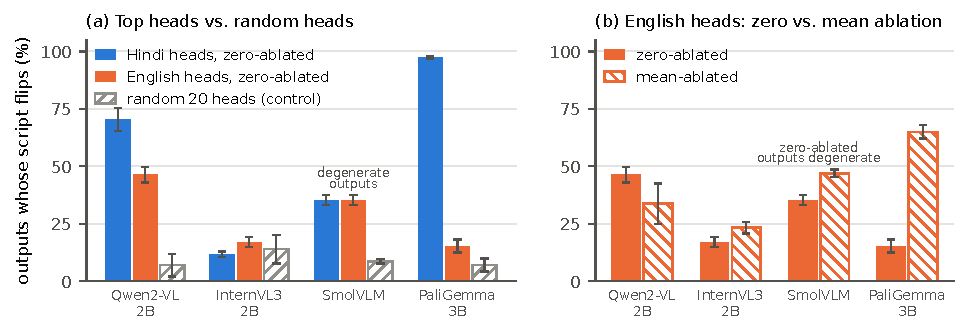
\includegraphics[width=\linewidth]{figures/ablation_bars.pdf}
\caption{Does ablating the top heads change output script? Percent of Hindi-English code-switched generations whose output script flips, as mean $\pm$ standard deviation over three seeds (Table~\ref{tab:seeds}). (a) Zero-ablating each model's top-20 Hindi or English heads, against 20 random heads. Qwen2-VL-2B and PaliGemma-3B clear the control by a wide margin. SmolVLM's zero-ablated outputs are degenerate, so its flips do not measure redirection. InternVL3-2B stays at the control level. (b) For English heads, mean ablation flips more outputs than zero ablation in PaliGemma-3B and fewer in Qwen2-VL-2B and InternVL3-2B; SmolVLM's comparison is uninformative.}
\label{fig:ablation}
\end{figure}

\paragraph{Clear effects: Qwen2-VL-2B and PaliGemma-3B.}
In these two models, zero-ablating the top Hindi heads flips the output script far more often than ablating random heads: 70.3 $\pm$ 5.0\% against 7.0 $\pm$ 4.9\% for Qwen2-VL-2B, and 97.3 $\pm$ 0.5\% against 7.0 $\pm$ 2.8\% for PaliGemma-3B, about fourteen times its control. The single run agrees, with bootstrap 95\% intervals that do not overlap the control (Qwen2-VL-2B 74\% [65,82] against 9\% [4,15]; PaliGemma-3B 97\% [93,100]). In that run PaliGemma-3B's random-head draw flipped an unusually high 31\% of outputs, against 5\%, 5\%, and 11\% in the three reseeded draws, so we use the seed means as the control. The English heads have a clear but smaller effect in Qwen2-VL-2B (46.3 $\pm$ 3.4\%) and a modest one in PaliGemma-3B (15.3 $\pm$ 2.9\%).

\paragraph{Ablation breaks generation: SmolVLM.}
SmolVLM's Hindi and English zero-ablations flip exactly the same outputs in every seed (38, 35, and 33 of 100), and those are exactly the outputs that were in Devanagari before ablation. With the heads removed, SmolVLM produces degenerate text (for example repeated \texttt{<row\_2>} tokens), which no longer contains Devanagari. Its 35.3\% flip rate is therefore its baseline Devanagari rate: the heads matter for generation, but the flip metric carries no information about which script they route.

\paragraph{No distinguishable effect: InternVL3-2B.}
InternVL3-2B's Hindi heads flipped 14\% of generations against a 9\% control in the single run. Across three seeds the effect disappears: hi-zero is 11.7 $\pm$ 1.2 against a random-head control of 14.0 $\pm$ 6.2. Its English heads fare slightly better (17.0 $\pm$ 2.2 against the same control) but not clearly. For this model we cannot distinguish ablating the top heads from ablating random ones.

\paragraph{The model with the most shared heads shows the weakest effect.}
If text and image inputs used the same heads, one would expect ablating heads found on text to disturb image-based generation most in that model. InternVL3-2B, whose Hindi heads overlap most across modalities (Section~\ref{sec:overlap}), shows the opposite. We see two candidate explanations and cannot yet decide between them. First, the flip metric only registers a switch to the other script (Section~\ref{sec:ablation_method}); if ablating shared heads damages generation without redirecting it, the damage would not show up as flips. Second, InternVL3-2B may spread language routing across more heads than the top 20, so that removing 20 of them leaves enough of the rest to keep the output script unchanged. SmolVLM shows that the first kind of failure does occur in this setting. Measuring generation quality under ablation (for example character error rate against the rendered sentence, repetition, and output length) and ablating larger head sets would separate these explanations.

\paragraph{Mean ablation versus zero ablation.}
For Qwen2-VL-2B and InternVL3-2B, mean-ablation of the English heads is gentler than zero-ablation (33.7 vs.\ 46.3\%, and 23.3 vs.\ 17.0\% for InternVL3-2B, whose zero-ablation is at control level), as expected if part of the zero-ablation effect is generic degradation rather than language-related suppression. PaliGemma-3B shows the reverse: mean-ablating its English heads flips 65.0 $\pm$ 2.9\% of outputs against 15.3 $\pm$ 2.9\% for zero-ablation, and the single run agrees with non-overlapping intervals (61\% [51,70] vs.\ 18\% [11,26]). One possible reading is that the \emph{mean} activation of these heads pushes generation toward English, so substituting it redirects output where zeroing only removes signal. A ceiling also plays a part: 85\% of PaliGemma-3B's baseline outputs are already in Latin script, so zero-ablating English heads has little room to flip script. SmolVLM's mean-ablation also flips more than its zero-ablation (47.0 vs.\ 35.3\%), but since its zero-ablated outputs are degenerate, the comparison says nothing about routing.

\paragraph{Baseline script differences.}
Without any ablation, SmolVLM produces Devanagari script far more often than the other models (37 of 100 outputs, against 5 for Qwen2-VL-2B, 11 for InternVL3-2B, and 15 for PaliGemma-3B). This is not explained by competence: SmolVLM is the weakest model on Hindi by character-normalized perplexity (Table~\ref{tab:competence}). We report it as a difference in decoding behavior that we do not explain.

\paragraph{Spanish-English.}
Spanish and English share Latin script, so we score a \emph{language} flip instead. We run a language identifier (\texttt{langid}, es vs.\ en) on the generated text for 100 Spanish-English images and check whether its dominant language changes from the un-ablated baseline (Table~\ref{tab:es_ablation}). Ablating the top heads flips the output language more often than the random-head control in every model, clearly for PaliGemma-3B (85\% and 82\% against 19\%) and by a smaller margin for Qwen2-VL-2B (17\% and 14\% against 8\%) and InternVL3-2B (48\% and 53\% against 33\%). SmolVLM's large rates (39\% and 51\%) most likely reflect the same breakdown of generation as for Hindi-English, which a language identifier would also register as a change. The es-head and en-head effects are much closer to each other than the hi-head and en-head effects are for Hindi-English, consistent with Spanish and English sharing script and much vocabulary. \texttt{langid} is also noisy on short code-switched generations, which raises the random-head control (up to 33\% for InternVL3-2B), so we read these as effects relative to each model's own control.

\begin{table}[t]
\centering
\caption{Spanish-English ablation. Percent of 100 es-en generations whose dominant language (\texttt{langid}, es vs.\ en) flips from the un-ablated baseline, zero-ablating the top-20 heads for Spanish or for English, against the random-head control. The control is raised by language-ID noise on short generations.}
\label{tab:es_ablation}
\begin{tabular}{l ccc}
\toprule
Model & es-heads & en-heads & Random-20 \\
\midrule
Qwen2-VL-2B  & 17\% & 14\% & 8\% \\
InternVL3-2B & 48\% & 53\% & 33\% \\
SmolVLM      & 39\% & 51\% & 8\% \\
PaliGemma-3B & \textbf{85\%} & \textbf{82\%} & 19\% \\
\bottomrule
\end{tabular}
\end{table}

\subsection{Exploratory: head positions and decoder family}
\label{sec:lineage}

Within each model, most of the top-20 text-condition heads are shared across all three languages. Qwen2-VL-2B shares 18 of 20, InternVL3-2B 14 of 20, SmolVLM 14 of 20, and PaliGemma-3B 15 of 20. Most heads that LAHIS ranks highly are therefore language-\emph{general}, consistent with what the score measures (Section~\ref{sec:lahis}).

Across models, we compared the (layer, head) positions of each model's top-20 text-condition heads. Figure~\ref{fig:lineage} shows the counts. Qwen2-VL-2B and InternVL3-2B, which have different vision encoders but decoders from the same family, share 18 of their 20 positions (a raw count; Jaccard $18/22 \approx 0.818$). Every other pair shares fewer. PaliGemma-3B shares 8 positions with Qwen2-VL-2B and 9 with InternVL3-2B, SmolVLM shares 2 and 1, and SmolVLM and PaliGemma-3B share none. All shared positions lie in the first two layers. The ordering does not follow language competence: even for English, where SmolVLM's competence is within 10\% of the Qwen pair (char-ppl 2.23 against 2.04--2.06), it shares only 2 and 1 English top-20 positions against the Qwen pair's 13. Nor does it follow the vision encoder: PaliGemma-3B and SmolVLM use the same SigLIP-SO400M family but share no positions.

\begin{figure}[t]
\centering
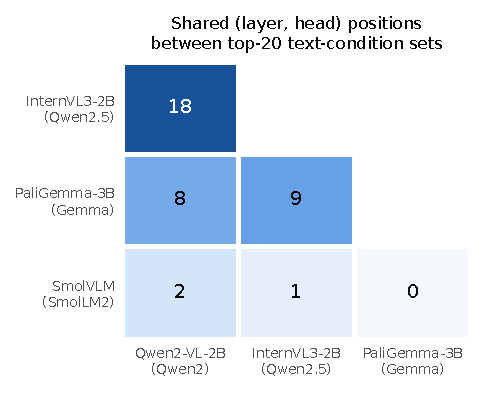
\includegraphics[width=0.5\linewidth]{figures/lineage_matrix.pdf}
\caption{Number of (layer, head) positions shared between each pair of models' top-20 text-condition heads, with each model's decoder family in parentheses. We report this as a description only: head numbering is not comparable across independently trained models, and the Qwen pair's 18 is largely expected from both placing their top heads in layers 0--1 (Section~\ref{sec:lineage}).}
\label{fig:lineage}
\end{figure}

We treat this as a description rather than a finding, for four reasons.
\begin{itemize}
    \item \textbf{Head numbering is arbitrary across independently trained models.} Heads within a layer are interchangeable, so the index ``head 3 of layer 0'' only refers to comparable units if two models share weights or initialization. None of our decoders share weights, including Qwen2 and Qwen2.5 (Section~\ref{sec:models}).
    \item \textbf{Most of the same-family match is expected from layer placement alone.} All 18 positions shared by Qwen2-VL-2B and InternVL3-2B lie in layers 0--1, which hold only 24 heads, so each model places at least 18 of its top 20 heads there. Two sets of 18 drawn from the same 24 positions must share at least 12, whatever the numbering, and would share about 13.5 if placed at random within those layers. The observed 18 is only modestly above that.
    \item \textbf{Decoder family is confounded} with head count, grid shape, attention scheme, and image compression in our four models.
    \item \textbf{The comparison rests on one same-family pair.}
\end{itemize}
What does survive these caveats is a layer-level pattern: the top text-condition heads of both Qwen-family models concentrate in the first two layers. Comparing how many top heads each model places in each layer does not depend on head numbering, and is the sounder basis for this question in future work.

% ============================================================
\section{What we can and cannot conclude}
\label{sec:conclusions_table}

Table~\ref{tab:claims} summarizes each observation, the evidence behind it, and how strongly we think that evidence supports it. \emph{Supported} means consistent evidence with a matched control; \emph{tentative} means one model, one language, or overlapping intervals; \emph{descriptive} means a pattern we report but cannot test with this design.

\begin{table}[t]
\centering
\caption{Summary of observations and the strength of evidence for each, within the four models studied.}
\label{tab:claims}
\small
\begin{tabular}{>{\raggedright\arraybackslash}p{0.38\linewidth} >{\raggedright\arraybackslash}p{0.38\linewidth} >{\raggedright\arraybackslash}p{0.14\linewidth}}
\toprule
Observation & Evidence & Strength \\
\midrule
Script identity is linearly decodable from the first vision-encoder layer, in all four models & Per-layer probes; transliteration control (Section~\ref{sec:probes}) & Supported \\
\addlinespace
Qwen2-VL-2B and SmolVLM use largely different heads for text and image input & Jaccard overlap above chance; stable across $K$ (Section~\ref{sec:overlap}) & Supported (single run) \\
\addlinespace
InternVL3-2B uses nearly the same heads for Hindi text and Hindi images & One model, one language (Section~\ref{sec:overlap}) & Tentative \\
\addlinespace
PaliGemma-3B shares or separates heads & Overlap near its chance level (Section~\ref{sec:overlap}) & Inconclusive \\
\addlinespace
Top heads (identified on monolingual text) redirect output script when reading code-switched images & Ablation vs.\ random control, three seeds, bootstrap CIs, in Qwen2-VL-2B and PaliGemma-3B (Section~\ref{sec:ablation}) & Supported for two models \\
\addlinespace
The same holds for SmolVLM & Ablation produces degenerate output; flips equal its baseline Devanagari rate (Section~\ref{sec:ablation}) & Not informative \\
\addlinespace
The same holds for InternVL3-2B & Effect within the control's spread across seeds (Section~\ref{sec:ablation}) & Not supported \\
\addlinespace
Top heads affect output language in Spanish-English & Above control in all models; noisy language ID (Section~\ref{sec:ablation}) & Tentative \\
\addlinespace
Mean ablation of English heads flips more outputs than zero ablation & PaliGemma-3B only, seeds and CIs agree; ceiling effect (Section~\ref{sec:ablation}) & Tentative \\
\addlinespace
Important head positions follow decoder family & Four models, one same-family pair; numbering not comparable; match largely expected from layer placement (Section~\ref{sec:lineage}) & Descriptive \\
\bottomrule
\end{tabular}
\end{table}

Two practical points follow even from the more cautious rows. First, one VLM's language heads cannot be assumed to be another's: the four models differ in whether text and image inputs share heads, in how strongly their encoders separate scripts, and in how their output responds to ablation. Second, a flip rate on its own can mislead: in SmolVLM, ablation produced what looked like a clean 35\% script effect but was in fact broken output, and in PaliGemma-3B mean and zero ablation disagreed sharply. Head-ablation studies should report output quality and both ablation types alongside the flip rate.

% ============================================================
\section{Limitations}
\label{sec:limitations}

\paragraph{Model scale and number.}
All four models are in the 1.7--3B range, a compute constraint rather than a scientific choice. Whether any of the patterns hold at 7--8B scale, or in other small VLMs, is untested.

\paragraph{Heads are identified on monolingual text.}
The head sets come from monolingual sentences, so RQ1 compares text and image processing of single-language content, and code-switching enters only through the probes and the ablation test. Scoring heads on the code-switched sentences themselves, for example with the loss restricted to Hindi or English tokens using the gold token labels, would tie the head sets to code-switched input directly.

\paragraph{What LAHIS and the flip metric measure.}
LAHIS ranks heads by their effect on next-token loss, so its top heads include language-general ones (Section~\ref{sec:lahis}), and the English and Hindi top-20 sets overlap heavily. The script-flip metric has no fluency control: it registers broken output as a flip whenever the broken output drops the original script, as it does for SmolVLM (Section~\ref{sec:ablation}). Both limit how directly our results speak to language routing specifically.

\paragraph{Run-to-run stability.}
The ablation flip rates are repeated across three seeds, each with a fresh sample of 100 sentences and a fresh random-head draw (Appendix~\ref{app:seeds}). The head-overlap values are single-run, controlled only by the permutation baseline.

\paragraph{Covarying architecture.}
Decoder family covaries with head-grid shape, head count, attention scheme, and image compression, none of which we vary independently. PaliGemma-3B's small $18 \times 8$ grid also raises its chance overlap (Table~\ref{tab:overlap}).

\paragraph{Two language pairs.}
With only Hindi-English and Spanish-English, we cannot separate script distance from language-family distance as the driver of InternVL3-2B's Hindi-specific overlap. The corpus is also imbalanced (806 vs.\ 127), though LAHIS uses a matched per-language sample, so this affects only the diversity of the Spanish-English ablation stimuli.

% ============================================================
\section{Conclusion}
\label{sec:conclusion}

We investigated whether small VLMs rely on the same attention heads for a language when it arrives as text tokens and as a rendered image, and whether those heads matter when the models read code-switched text. In the four models we studied, the answer depends on the model. Two use largely different heads for the two inputs, one uses nearly the same heads but only for Hindi, and for one our measure cannot tell. Every vision encoder makes script identity available from its first layer, so these differences do not come from the encoders failing to separate scripts. Ablating the top heads while the models read code-switched images redirects the output script far beyond a random-head control in two models. In a third, ablation breaks generation instead, and in the model whose text and image heads overlap most, the effect is indistinguishable from the control, a result we cannot yet explain. Future work could identify heads on code-switched text directly, measure output quality alongside script flips, compare head placement at the layer level across models, and extend the analysis to larger VLMs and to language pairs that separate script from language family.

% ============================================================
\bibliography{references}
\bibliographystyle{tmlr}

% ============================================================
\clearpage
\appendix


\section{Full Overlap Values}
\label{app:overlap}

\begin{table}[H]
\centering
\caption{Jaccard overlap of top-20 heads across conditions. A = text, B = image+query, C = image-only. Lang is the language of the monolingual FLORES sentences used to compute the LAHIS scores (Section~\ref{sec:data}). Chance ($p_{95}$): 0.081 (Qwen2-VL-2B, InternVL3-2B), 0.053 (SmolVLM), 0.143 (PaliGemma-3B, whose small $18 \times 8$ head grid raises its chance level).}
\label{tab:overlap}
\begin{tabular}{ll ccc}
\toprule
Model & Lang & $\AcapB$ & $\AcapC$ & $\BcapC$ \\
\midrule
\multirow{3}{*}{Qwen2-VL-2B}
  & en & 0.143 & 0.081 & 0.538 \\
  & es & 0.081 & 0.053 & 0.538 \\
  & hi & 0.111 & 0.176 & 0.429 \\
\midrule
\multirow{3}{*}{InternVL3-2B}
  & en & 0.333 & 0.176 & 0.176 \\
  & es & 0.538 & 0.250 & 0.212 \\
  & hi & \textbf{0.905} & \textbf{0.667} & 0.667 \\
\midrule
\multirow{3}{*}{SmolVLM}
  & en & 0.176 & 0.143 & 0.667 \\
  & es & 0.111 & 0.111 & \textbf{0.905} \\
  & hi & 0.250 & 0.212 & \textbf{0.905} \\
\midrule
\multirow{3}{*}{PaliGemma-3B}
  & en & 0.250 & 0.333 & 0.333 \\
  & es & 0.212 & 0.290 & 0.250 \\
  & hi & 0.250 & 0.290 & 0.333 \\
\bottomrule
\end{tabular}
\end{table}

\section{$K$-Sweep}
\label{app:ksweep}

Table~\ref{tab:ksweep} shows $\AcapC$ and $\BcapC$ at the two extremes of our $K \in \{5, 10, 20, 40, 80\}$ sweep, bracketing the $K{=}20$ values in Table~\ref{tab:overlap}. The full sweep (all five $K$ values, all four models, all three languages) is released with the code as \texttt{checkpoints/head\_overlap\_matrix.json}.

\begin{table}[H]
\centering
\caption{Text-image ($\AcapC$) vs.\ image-image ($\BcapC$) Jaccard overlap at $K{=}5$ and $K{=}80$, the two extremes of the sweep. Qwen2-VL-2B and SmolVLM keep $\AcapC$ well below $\BcapC$ at both extremes, for every language. InternVL3-2B's Hindi row keeps $\AcapC$ and $\BcapC$ close together at both extremes. PaliGemma-3B's overlaps sit uniformly higher ($\AcapC$ already 0.25 at $K{=}5$) because its small $18{\times}8$ head grid inflates chance-level Jaccard (Table~\ref{tab:overlap}); its $\AcapC$ and $\BcapC$ track each other loosely at both extremes, consistent with the inconclusive result at $K{=}20$.}
\label{tab:ksweep}
\begin{tabular}{ll cccc}
\toprule
Model & Lang & $\AcapC$@5 & $\AcapC$@80 & $\BcapC$@5 & $\BcapC$@80 \\
\midrule
\multirow{3}{*}{Qwen2-VL-2B}
  & en & 0.000 & 0.240 & 0.429 & 0.539 \\
  & es & 0.000 & 0.176 & 0.429 & 0.553 \\
  & hi & 0.111 & 0.240 & 0.667 & 0.650 \\
\midrule
\multirow{3}{*}{InternVL3-2B}
  & en & 0.000 & 0.301 & 0.111 & 0.468 \\
  & es & 0.000 & 0.301 & 0.000 & 0.416 \\
  & hi & \textbf{1.000} & 0.584 & \textbf{1.000} & 0.739 \\
\midrule
\multirow{3}{*}{SmolVLM}
  & en & 0.000 & 0.231 & \textbf{1.000} & 0.861 \\
  & es & 0.111 & 0.203 & \textbf{1.000} & 0.839 \\
  & hi & 0.000 & 0.368 & \textbf{1.000} & 0.882 \\
\midrule
\multirow{3}{*}{PaliGemma-3B}
  & en & 0.250 & 0.495 & 0.429 & 0.778 \\
  & es & 0.250 & 0.538 & 0.111 & 0.616 \\
  & hi & 0.250 & 0.468 & 0.250 & 0.667 \\
\bottomrule
\end{tabular}
\end{table}

\section{Single-Run Ablation Results}
\label{app:single}

Table~\ref{tab:ablation} reports the original single ablation run. Its bootstrap 95\% intervals (10{,}000 resamples over the 100 images) are quoted in Section~\ref{sec:ablation}.

\begin{table}[H]
\centering
\caption{Single run (random seed 42): \% of 100 Hindi-English code-switched generations whose output script flips from the un-ablated baseline, by ablation variant (top-20 heads for the named language). The four columns are Qwen2-VL-2B, InternVL3-2B, SmolVLM, and PaliGemma-3B. PaliGemma-3B's random-head draw in this run flipped 31\% of outputs, against 5--11\% in the three reseeded draws (Table~\ref{tab:seeds}), which we treat as the primary results. SmolVLM's zero-ablation flips reflect degenerate output (Section~\ref{sec:ablation}).}
\label{tab:ablation}
\begin{tabular}{l cccc}
\toprule
Variant & Qwen & Intern & Smol & PaliG \\
\midrule
Zero-ablate en & 53\% & 25\% & 37\% & 18\% \\
Zero-ablate hi & 74\% & 14\% & 37\% & \textbf{97\%} \\
Mean-ablate en & 33\% & 20\% & \textbf{52\%} & \textbf{61\%} \\
Mean-ablate hi & 29\% & 24\% & 18\% & 30\% \\
\midrule
Random-20 (control) & 9\% & 9\% & 9\% & 31\% \\
\bottomrule
\end{tabular}
\end{table}

\section{Seed Variance}
\label{app:seeds}

To check that the ablation flip rates are not an artifact of one stimulus sample, we repeat the Hindi-English ablation under three seeds. Each seed draws its own sample of 100 sentences from the 806 Hindi-English code-switched sentences and its own random 20-head control, and Table~\ref{tab:seeds} reports the mean and standard deviation of each flip rate. The standard deviations are small (at most 8.8 points, and below 5 for most cells). For Qwen2-VL-2B and PaliGemma-3B, the Hindi zero-ablation effect stays far above the random control under every seed. SmolVLM's Hindi and English zero-ablations flip the same outputs in every seed (38, 35, and 33), namely those that were in Devanagari before ablation (Section~\ref{sec:ablation}). For InternVL3-2B it does not: its hi-zero rate (11.7 $\pm$ 1.2) falls within the spread of its random control (14.0 $\pm$ 6.2), which is why Section~\ref{sec:ablation} reports no distinguishable effect for this model.

\begin{table}[H]
\centering
\caption{Hindi-English ablation flip rates (percent) as mean $\pm$ standard deviation across three seeds. hi-/en-zero and hi-/en-mean zero- and mean-ablate the top-20 heads scored on Hindi or English; random ablates 20 random heads outside those sets, redrawn per seed.}
\label{tab:seeds}
\begin{tabular}{l ccccc}
\toprule
Model & hi-zero & en-zero & random & hi-mean & en-mean \\
\midrule
Qwen2-VL-2B  & $70.3 \pm 5.0$ & $46.3 \pm 3.4$ & $7.0 \pm 4.9$  & $30.3 \pm 5.4$ & $33.7 \pm 8.8$ \\
InternVL3-2B & $11.7 \pm 1.2$ & $17.0 \pm 2.2$ & $14.0 \pm 6.2$ & $22.7 \pm 3.3$ & $23.3 \pm 2.5$ \\
SmolVLM      & $35.3 \pm 2.1$ & $35.3 \pm 2.1$ & $8.7 \pm 0.9$  & $23.3 \pm 3.3$ & $47.0 \pm 1.6$ \\
PaliGemma-3B & $97.3 \pm 0.5$ & $15.3 \pm 2.9$ & $7.0 \pm 2.8$  & $29.3 \pm 2.6$ & $65.0 \pm 2.9$ \\
\bottomrule
\end{tabular}
\end{table}

\section{LAHIS Head-Importance Maps}
\label{app:lahis}

Figure~\ref{fig:lahis_hi} shows the raw per-head LAHIS importance behind the overlap analysis, for Hindi, as a layer $\times$ head grid per model and condition. Qwen2-VL-2B's text importance (A) is confined to layers 0--1, while its image conditions (B, C) recruit heads throughout the depth, so the top-20 sets barely intersect. InternVL3-2B's A, B and C light up nearly the same early heads. SmolVLM's importance is sparse and scattered across its wide $24 \times 32$ grid. PaliGemma-3B's importance is spread diffusely across layers with no sharp concentration, so its top-20 sets overlap only at the chance level its small $18 \times 8$ grid dictates.

\begin{figure}[p]
\centering
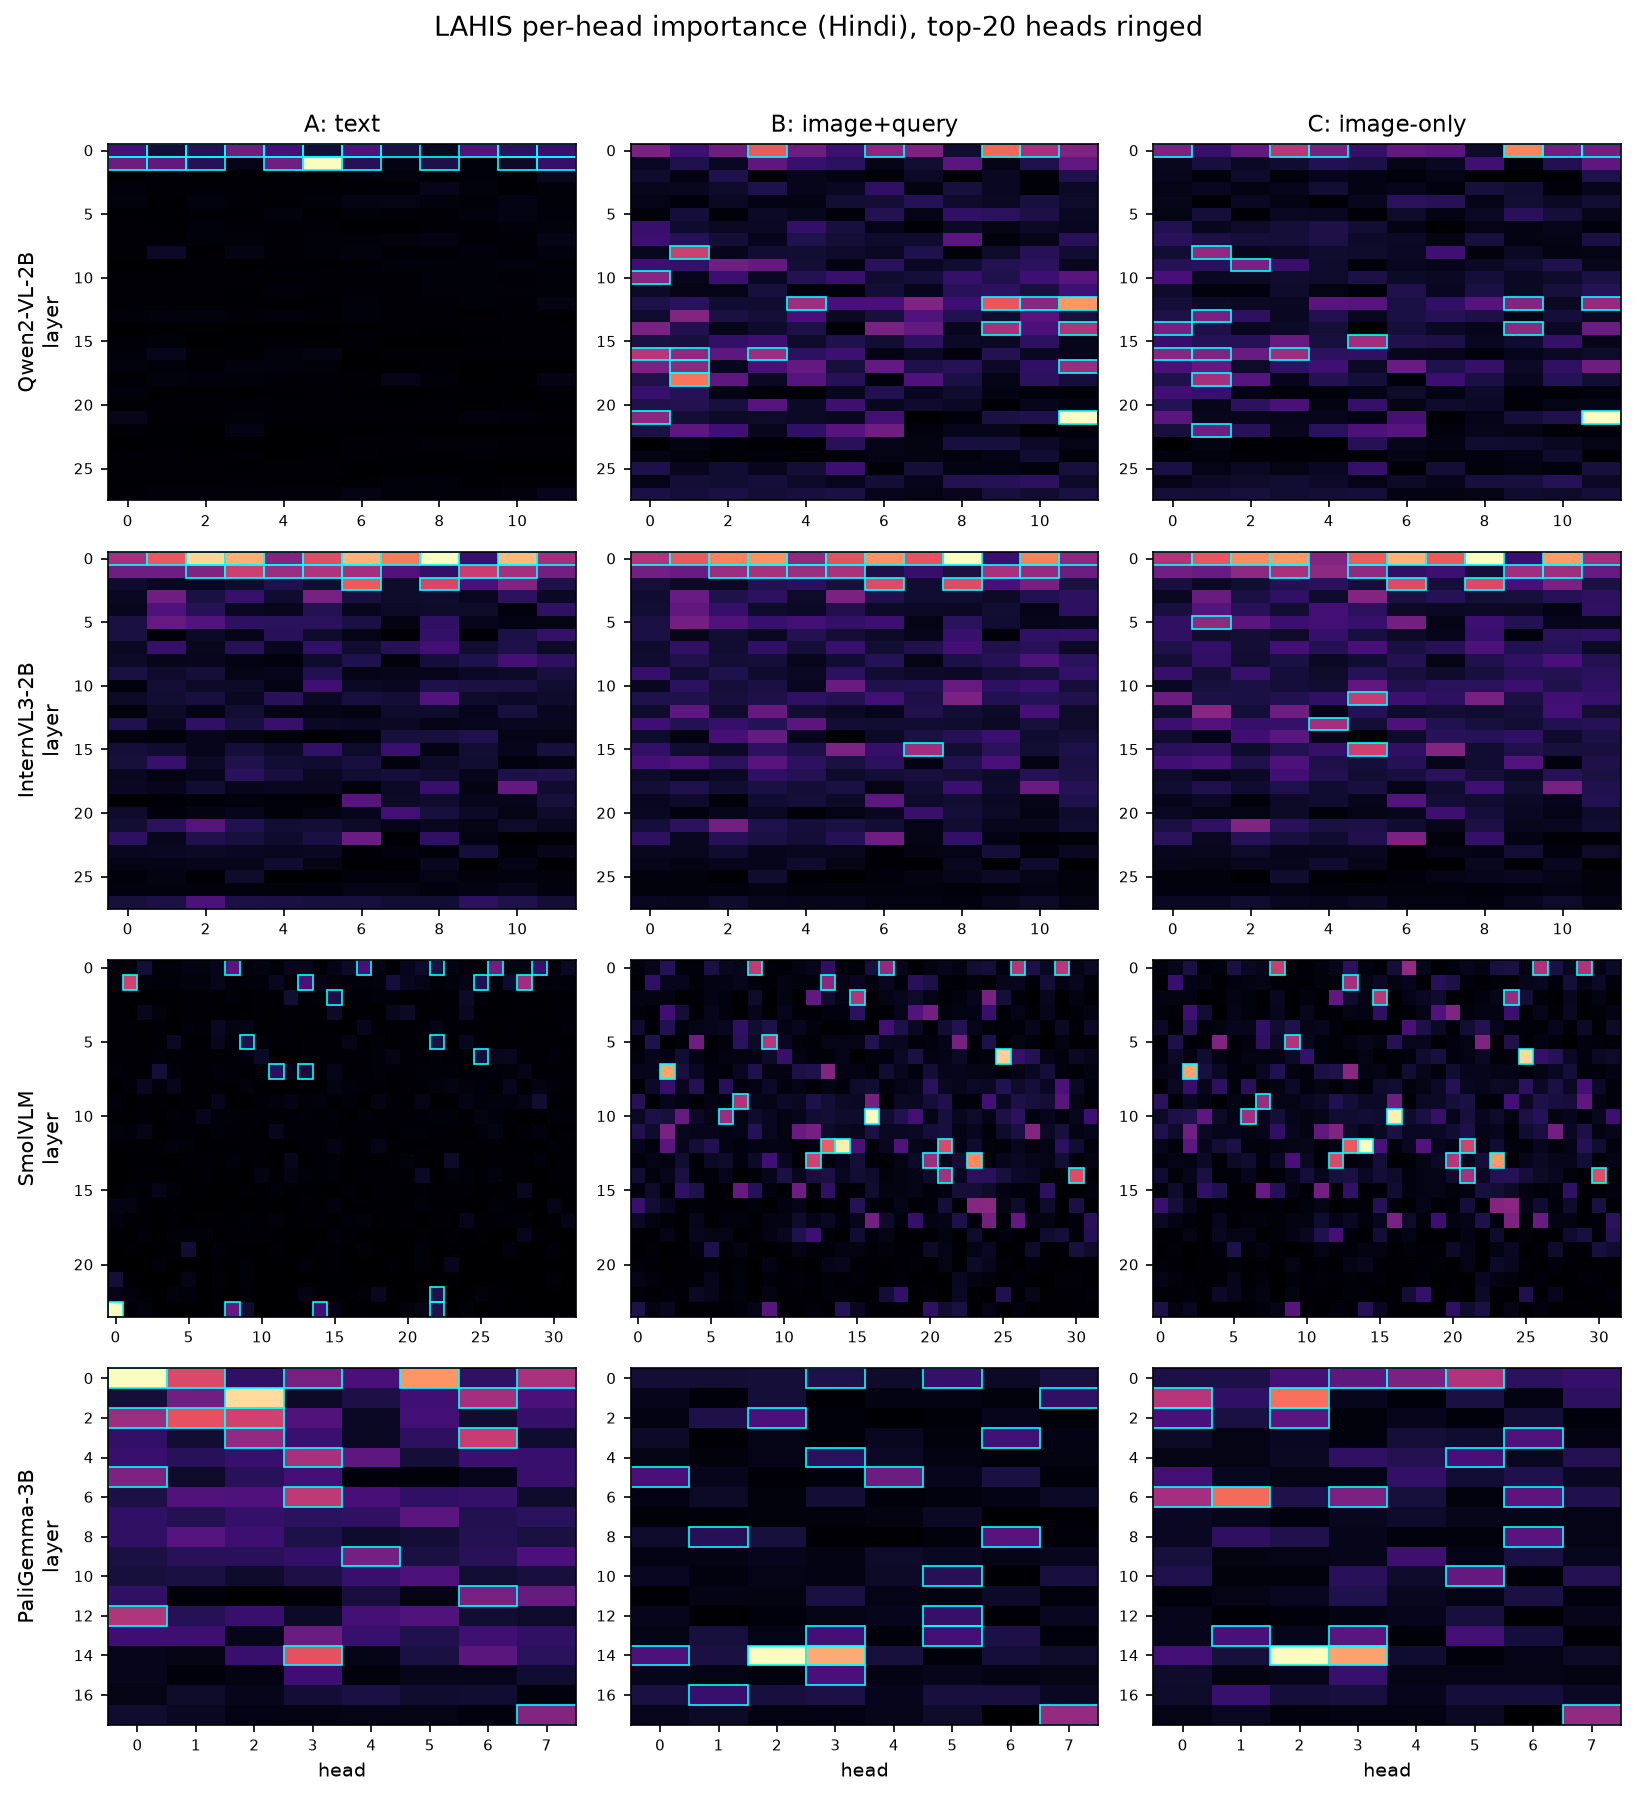
\includegraphics[width=0.95\linewidth]{figures/lahis_hindi.png}
\caption{LAHIS per-head importance for Hindi, min-max normalized within each panel. Rows are the four models and columns the three routing conditions (A=text, B=image+query, C=image-only). Cyan rings mark each panel's top-20 heads (the set entering the overlap analysis). Grid shapes differ by model ($28{\times}12$, $28{\times}12$, $24{\times}32$, $18{\times}8$). Brighter is more important.}
\label{fig:lahis_hi}
\end{figure}

\begin{figure}[p]
\centering
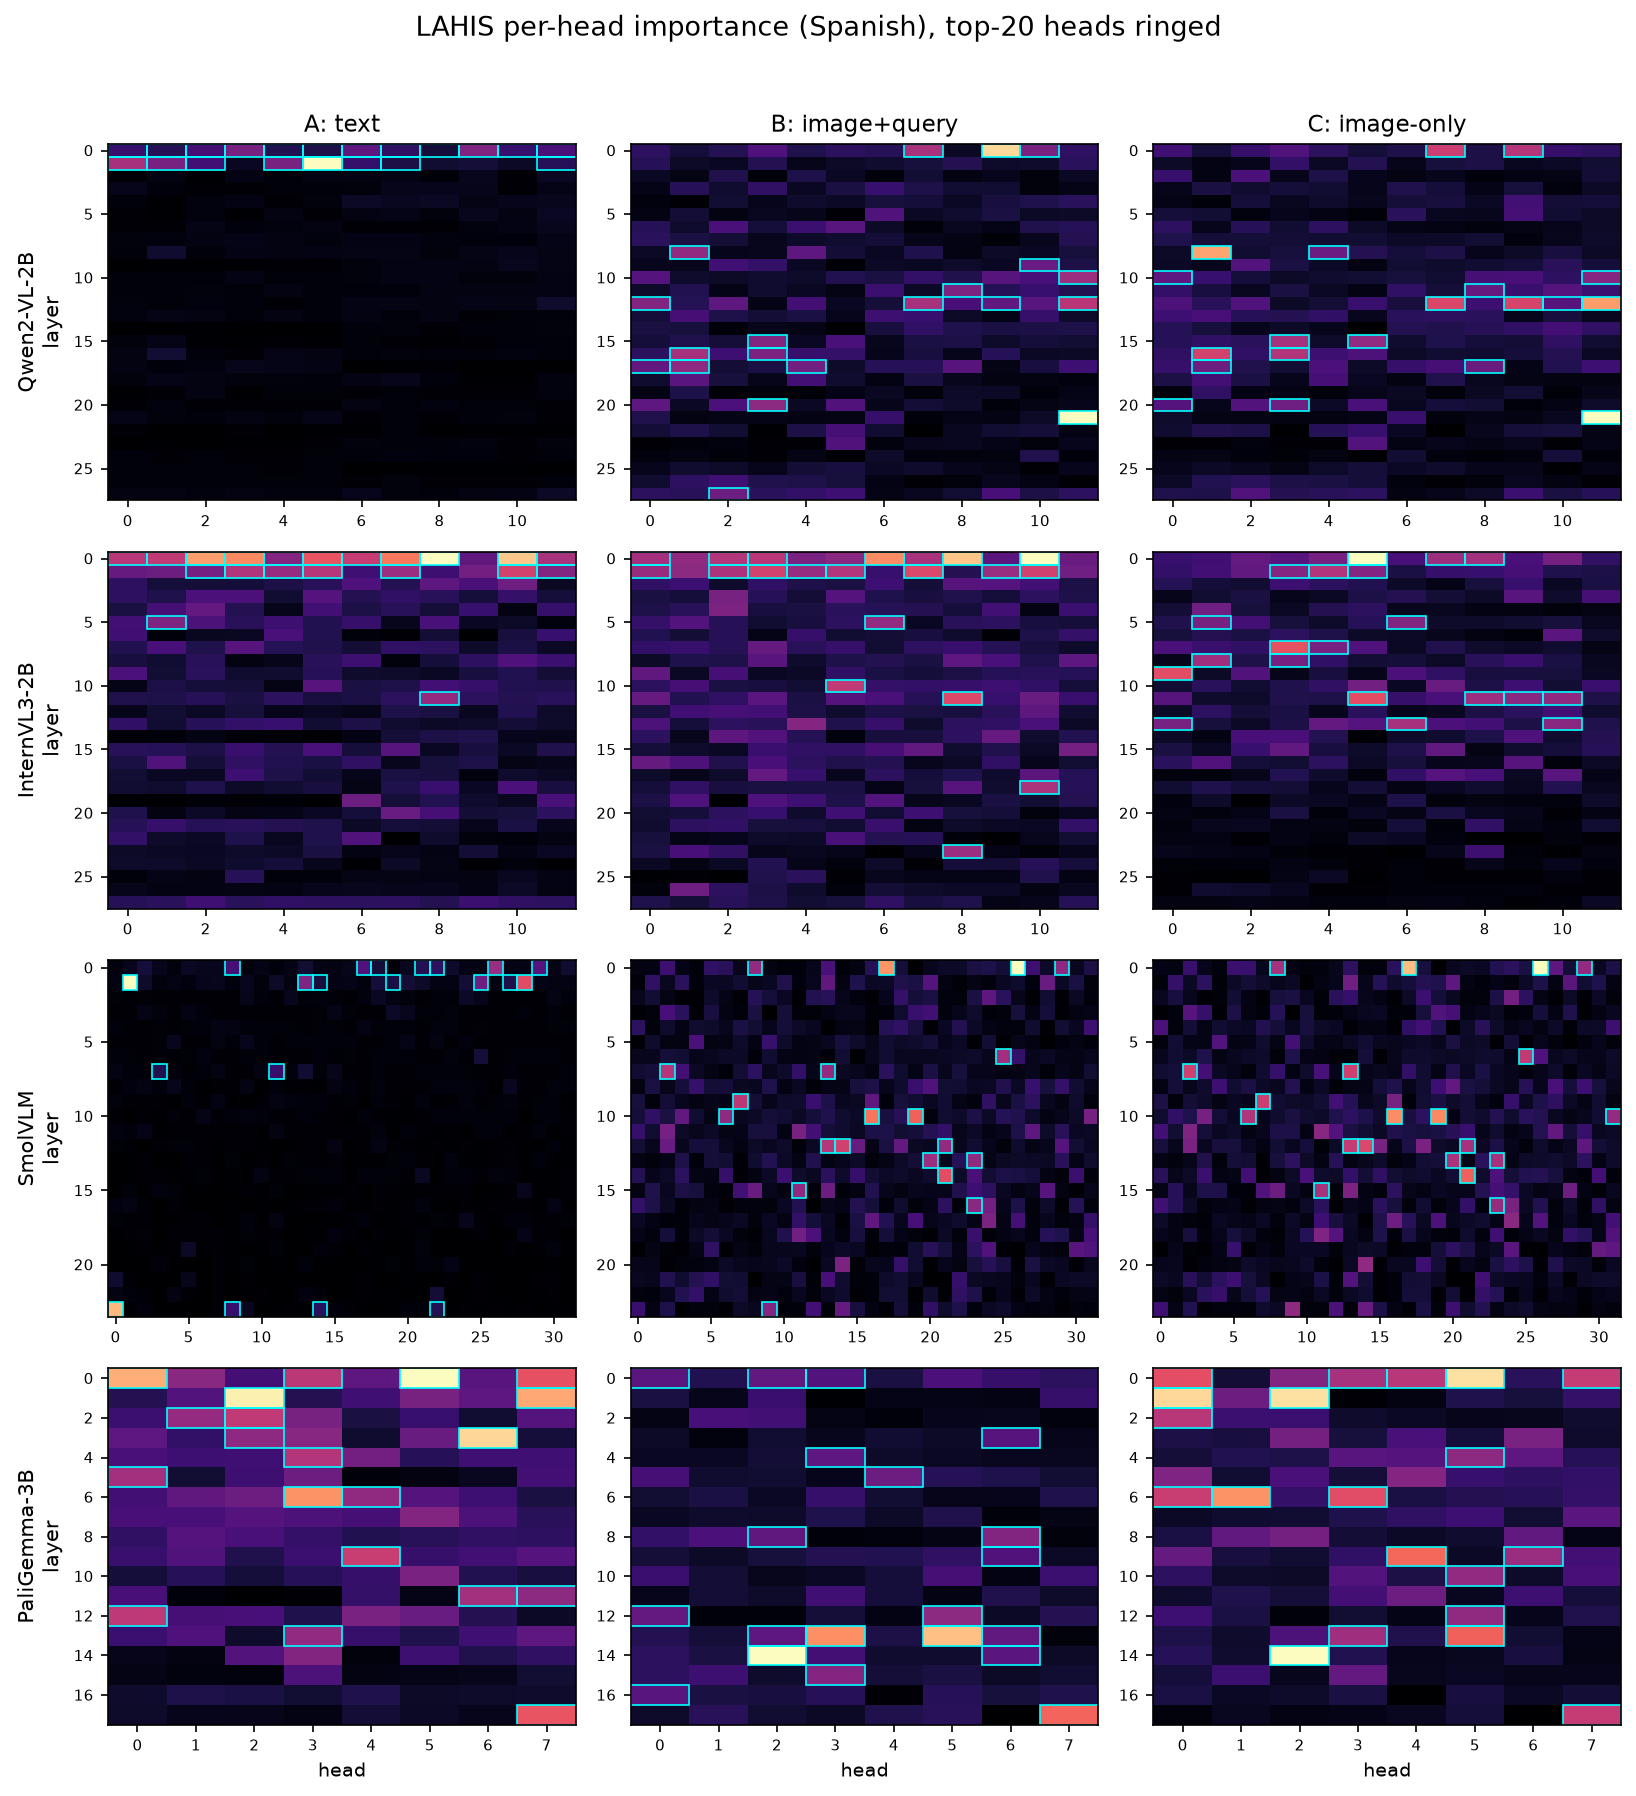
\includegraphics[width=0.95\linewidth]{figures/lahis_spanish.png}
\caption{LAHIS per-head importance for Spanish, plotted as in Figure~\ref{fig:lahis_hi} (rows are the four models, columns the three routing conditions, cyan rings mark each panel's top-20 heads). The important heads sit in the same layer bands as for Hindi, but for InternVL3-2B the text and image panels align less closely than they do for Hindi, consistent with its lower Spanish text-image overlap in Table~\ref{tab:overlap}.}
\label{fig:lahis_es}
\end{figure}


\end{document}
